\chapter{Current Work}\label{ch:current}

\section{\Cyclus}

The \Cyclus framework discussed in chapter \ref{ch:paradigm} provides a fuel 
cycle simulation platform on which to initially develop and deploy the 
repository model that is the subject of this effort. As a part of this effort 
also under development, \Cyclus has been developed with an architecture that 
supports the goals of this effort and will continue to mature in parallel with 
the development of this model.

\subsection{Available Models}

\Cyclus has a base set of models that are currently available and will support 
open and some closed fuel cycle simulations. These include a source and a sink 
facility model as well as recipe based reactor models, an enrichment facility, 
an intermediate storage facility, and a fleet of markets that direct material 
movement in the simulation.

Further fuel cycle facility models are being developed within \Cyclus  that 
will be essential for providing interesting scenarios for comparison via 
repository metrics. For a modified open cycle, a separations facility is 
necessary that will be capable of conducting arbitrarily complex chemical 
separations of used fuel. Similarly, an associated reprocessing facility  will 
be neccessary that is equipped to handle the so called `winery' problem of 
constructing critical fresh fuel assemblies appropriate for specific reactors 
from separated streams.


\section{GDSM Analysis}

Much of my future work is based on the parametric and regression analysis that
has begun with the base case Clay \gls{GDSM} at \gls{ANL}.

\subsection{Sensitivity Analyses}

The Used Fuel Cycle Division has reported sensitivity results for various 
parameters as they affect Peak PeakMean Annual Dose. Current work has involved a cursory  
exploration of other parameters within the Clay \gls{GDSM} as well. Current 
efforts to repeat those calculations for source term rather than 
dose will provide some insight for the sensitivity of subcomponent models to the 
parameters discussed below. This preliminary analysis has focused on general 
trends and coefficients defining the relationships between these 
parameters and source term over time for each isotope. 

\subsubsection{Cooling Time}

Extending the cooling time between discharge and emplacement results
in an altered waste stream. The resulting source term releases
of this waste stream were expected to differ from base case results. 
Nonetheless it was found that for the clay \gls{GDSM} there was approximately 
no Peak Annual Dose sensitivity to the cooling period length 
\cite{clayton_generic_2011}.

\begin{figure}[h!]
  \begin{center}
    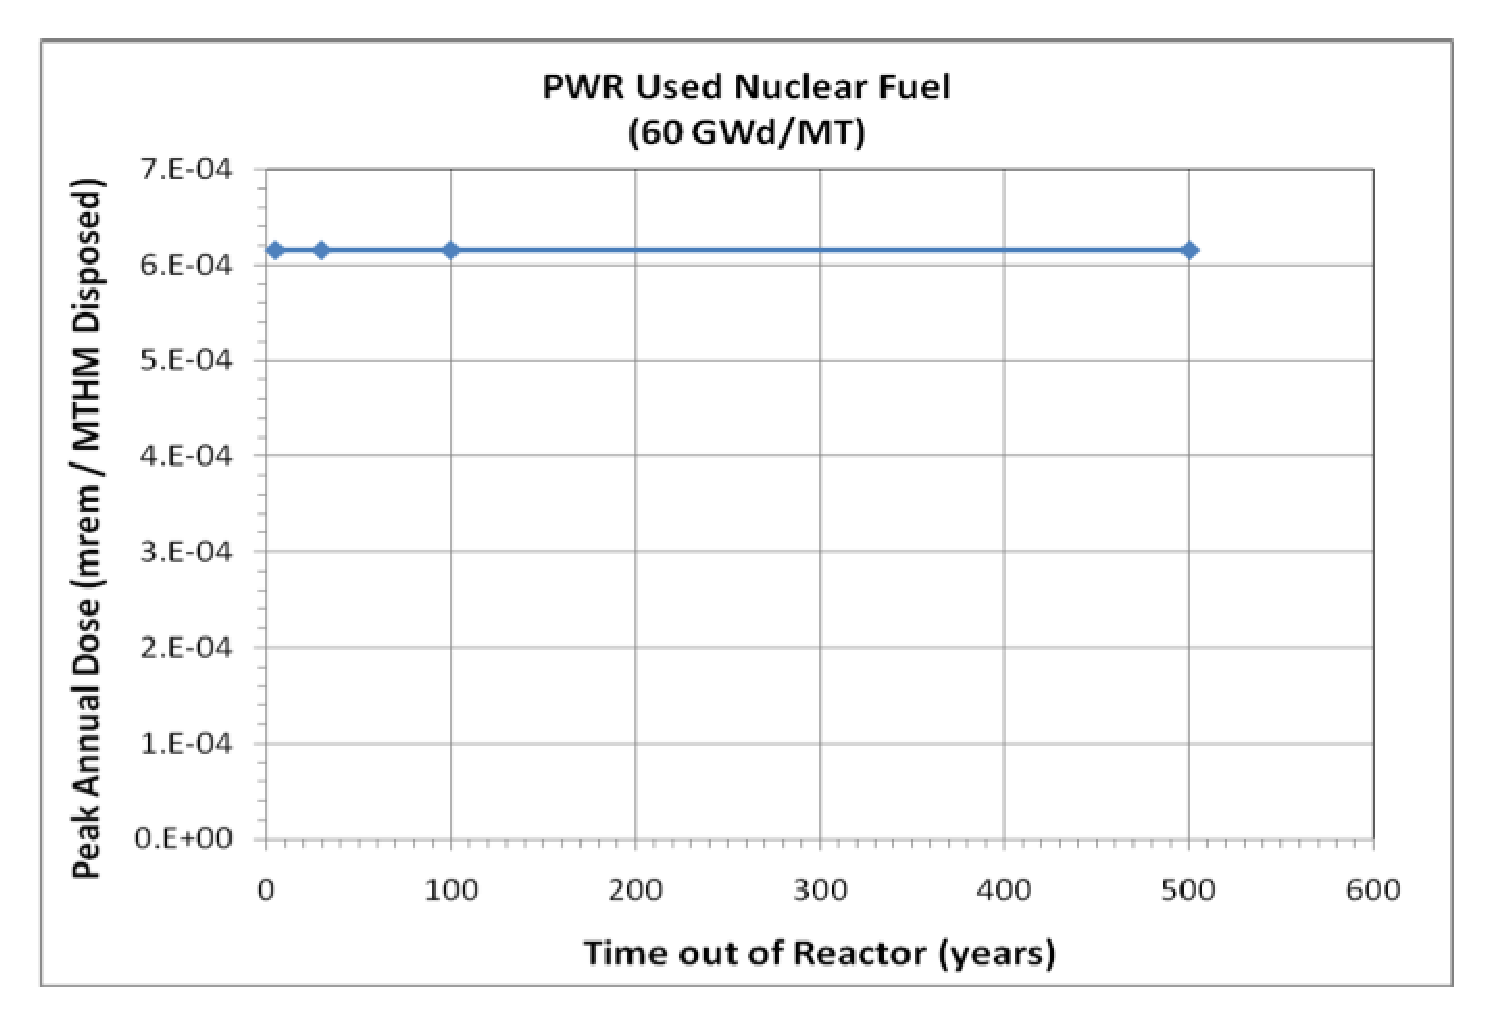
\includegraphics[height=7cm]{./chapters/current/coolingTime.eps}
  \end{center}
  \caption{An analysis by the UFD campaign with the clay GDSM shows that
  the peak annual dose is not sensitive at all to the cooling time of a 60GWd 
  burnup PWR fuel \cite{clayton_generic_2011}.}
  \label{fig:coolingTime}
\end{figure}

\clearpage 

\subsubsection{Burnup}

The burnup of a used fuel assembly results in an altered waste stream at the 
time of emplacement. It was found that for the clay \gls{GDSM}, the mean 
annual dose sensitivity to waste form dissolution rate became more important 
linearly with increased burnup \cite{clayton_generic_2011}.


\begin{figure}[h!]
  \begin{center}
    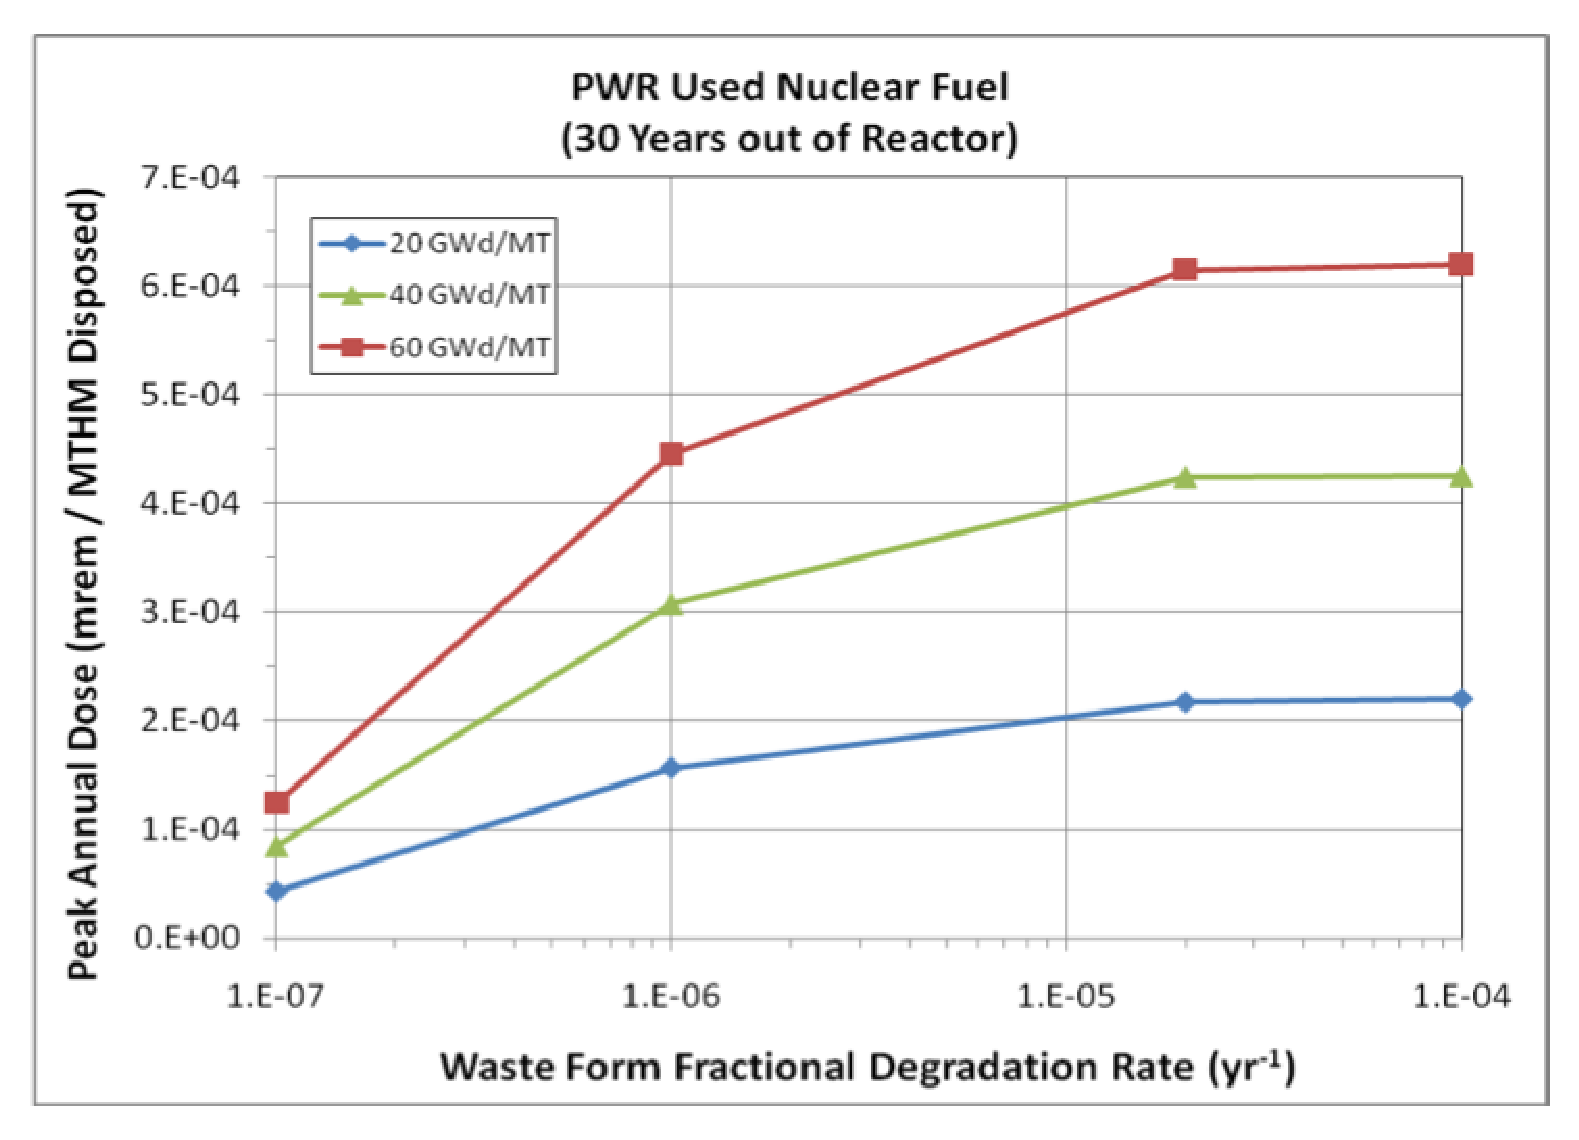
\includegraphics[height=7cm]{./chapters/current/BUandWPdeg.eps}
  \end{center}
  \caption{An analysis by the UFD campaign with the clay GDSM shows that
  the peak annual dose is more sensitive to waste package degradation rate with 
  increased burnup\cite{clayton_generic_2011}.}
  \label{fig:BUandWPdeg}
\end{figure}
\clearpage

\subsubsection{Drift Spacing}

The mean annual dose is not very sensitive to the horizontal spacing between 
drifts. 

\subsubsection{Vertical Distance to Aquifer}

The vertical distance to the aquifer above the disposal configuration defines 
the distance separating source term nuclide contaminants from the biospere. The 
clay model indicates that the mean annual dose is very sensitive to this 
distance \cite{clayton_generic_2011}.

\begin{figure}[h!]
  \begin{center}
    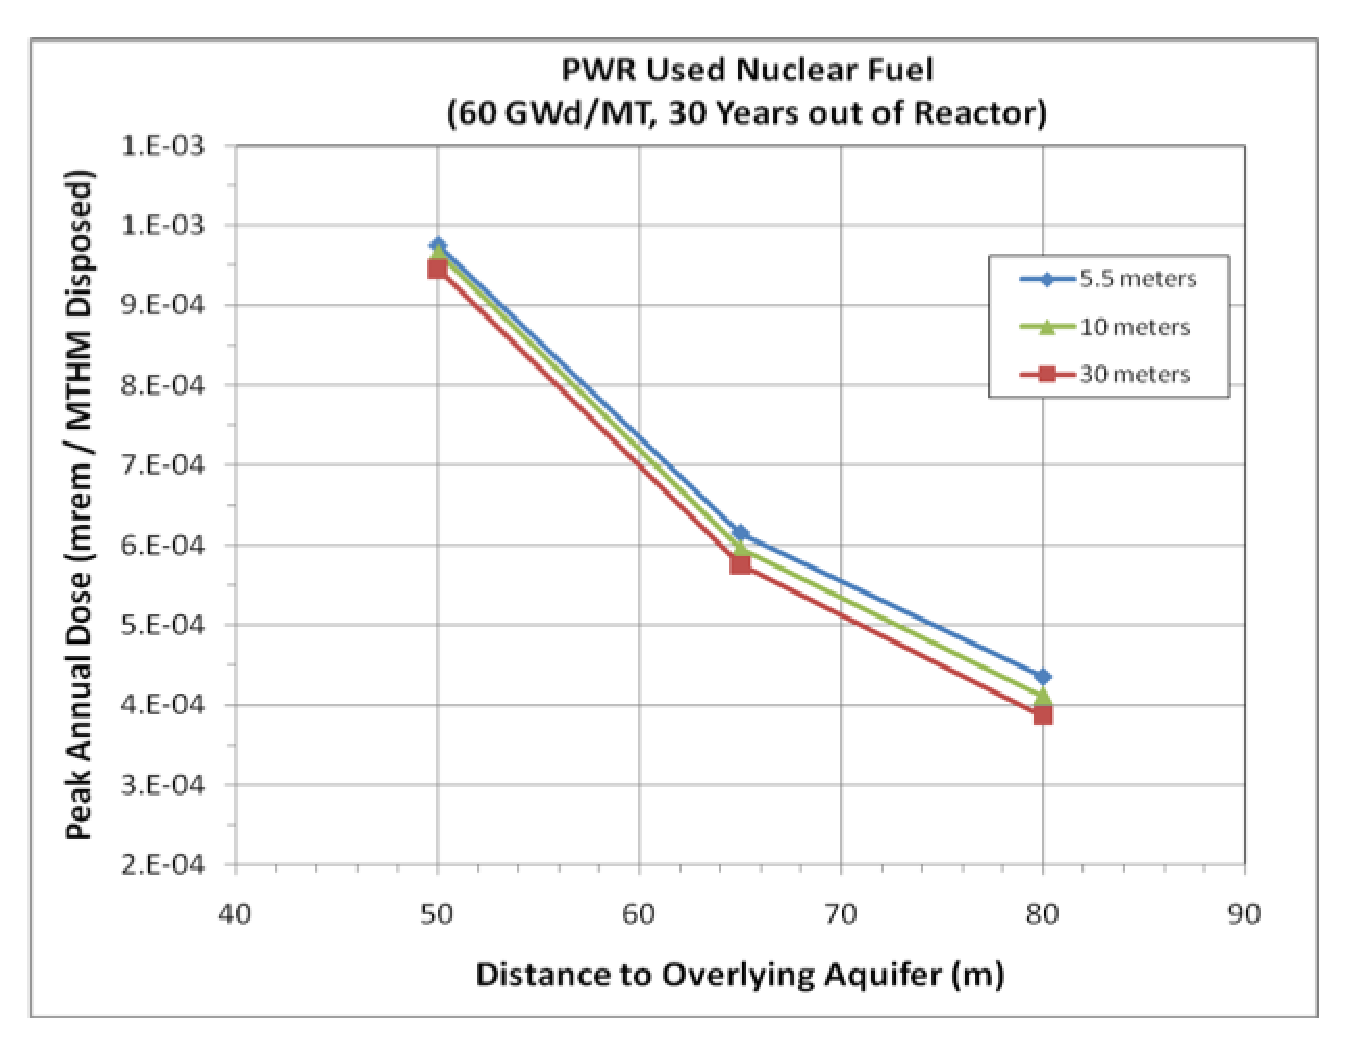
\includegraphics[height=7cm]{./chapters/current/overlyingDist.eps}
  \end{center}
  \caption{An analysis by the UFD campaign with the clay GDSM shows that 
  the peak annual dose is very sensitive to the distance to the overlying 
  aquifer\cite{clayton_generic_2001}.}
  \label{fig:overlyingDist}
\end{figure}
\clearpage


\subsubsection{Vertical Darcy Velocity}

Sensitivity to vertical Darcy velocity is similar to the sensitivity to vertical 
distance to aquifer in the sense that it directly determines the nuclide travel 
time to the biosphere. The clay model indicates that the mean annual dose is 
very sensitive to this parameter \cite{clayton_generic_2011}.


\begin{figure}[h!]
  \begin{center}
    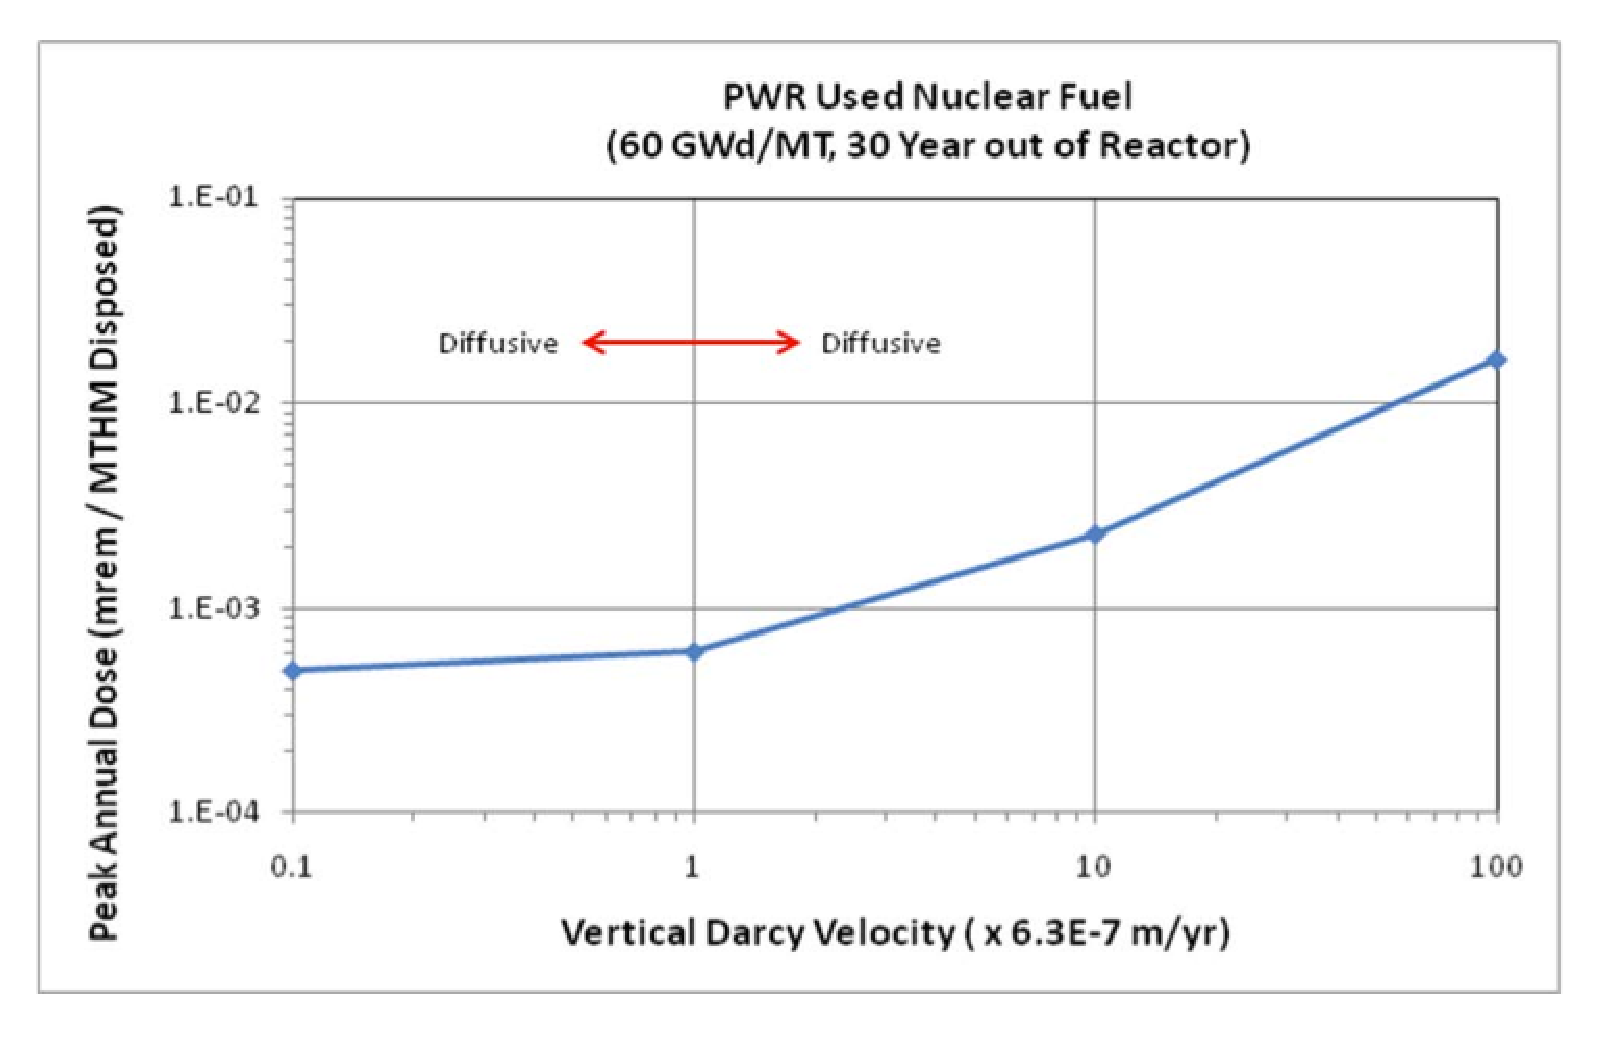
\includegraphics[height=7cm]{./chapters/current/vertDarcyVel.eps}
  \end{center}
  \caption{An analysis by the UFD campaign with the clay GDSM shows that 
  the peak annual dose is very sensitive to the vertical Darcy velocity  
  \cite{clayton_generic_2001}.}
  \label{fig:vertDarcyVel}
\end{figure}

It is assumed that the thermal model will not demonstrate any
sensitivity to the vertical Darcy velocity. Since heat dissipation in the far 
field is taken to be completely diffusive in clay, the Darcy velocity and the 
thermal model are entirely independent.

\clearpage

\subsubsection{Hypothetical Intersecting Fast Advective Pathway}

A fast pathway model intended to demonstrate a disrupted scenario is modeled as 
a single intersecting fracture in the clay matrix. The importance of the various 
ways in which this fast pathway intersects the model is very nuclide specific 
\cite{clayton_generic_2011}. In the clay model the fast pathway intersects the 
engineered barrier system either directly in the emplaced waste or just outside 
the secondary engineered barrier system.

It is assumed that the thermal model will not demonstrate any
sensitivity to the presence of a fast pathway. Since advective heat dissipation 
in such a crack would be minimal at the water speeds being considered. The 
thermal mocel takes the far field to be completely advective, also, and does not 
currently have the capability to model a fast pathway.

\subsubsection{Dimensions of Hypothetical Fast Pathway}

That is, how important is the crack width?

J Ahn's PhD  thesis had some analytical answers to this question.

\subsubsection{Permeable Porous Medium Porosity}

This should have a very slight linear effect. A coefficient needs to be derived 
from the relationship.

\subsubsection{Waste Form Degradation Rate}

This will be irrelevant for cases with low burnup or no fast pathway. 

\subsubsection{Waste Form Release Mode}

Solubility limited? Continuous?

\subsubsection{Waste Package Degradation Rate}

This will be irrelevant for cases with low burnup or no fast pathway. 

\subsubsection{Waste Package Release Mode}

Solubility limited? Continuous?

\subsubsection{Nuclide Solubilities}

For each nuclide.

\subsubsection{Etc. }

There are many parameters I haven't thought of.

\subsection{Comparison with other geologies}

A short comparison with each of the other models representing specific geologies 
will be begun in order to determine the differences in results for similar 
parameters.


\section{SINDA Model Analysis}
\subsection{Sensitivity Analysis}
\subsubsection{Cooling Time}

Extending the cooling time between discharge and emplacement results
in an altered waste stream. The emplacement capacity
of this waste stream may be expected to differ from base case results. 

Since the cooling period will be modeled outside of the repository model within  
the \Cyclus analysis, this sensitivity will not be incorporated into the 
repository modeling effort at the heart of this work, but gives an intuition for 
appropriate sensitivity to altered waste streams.

It is expected that the cooling time alters heat based capacity. 

<+sindaAnalysis+>

<+coolingVScapacityGRAPH+>

\subsubsection{Burnup}

It is expected that the burnup will significantly alter heat based capacity. 

<+sindaAnalysis+>

<+burnupVScapacityGRAPH+>

\subsubsection{Heat Generating Isotopes}

Plutonium and minor actinides are dominant contributors to heat. Focusing on
the sensitivity of the heat based capacity to the waste stream content of 
these nuclides could significantly simplify the heat analysis. 
 
For each of these, a sensitivity analysis of capacity to the nuclide will be 
developed by analyzing the thermal repository capacity for a waste stream of 
that nuclide alone.  

<+sindaAnalysis+>

<+contributorMassVSCapacityGRAPH+>

\subsubsection{Drift Spacing}

It is expected that the heat based capacity will be highly sensitive to the 
spacing between drifts. A higher drift density produces larger amounts of heat 
generation per repository footprint area. Constrained by heat limits typically 
at the drift tunnel boundaries, the repository capacity is reduced by increased 
areal loading density. 

<+sindaAnalysis+>

<+spacingVScapacityGRAPH+>

\subsubsection{Waste Package Separation}

It is expected that the heat based capacity will be highly sensitive to the 
spacing between packages linearly within the drifts. A higher line loading 
density produces larger amounts of heat generation per repository footprint 
area.  Again, the repository capacity is reduced by increased areal loading 
density. 

<+sindaAnalysis+>

<+lineloadingVScapacityGRAPH+>


\subsubsection{Waste Package Loading Density}

It is expected that the heat based capacity will be highly sensitive to the 
mass loading per waste package. A higher package loading density produces larger amounts 
of heat 
generation per repository footprint area. Constrained by heat limits typically 
at the drift tunnel boundaries, the repository capacity is reduced by increased 
areal loading density. 

<+sindaAnalysis+>

<+pkgloadingVScapacityGRAPH+>

\subsubsection{Clay Porosity}

It is expected that the heat based capacity will be fairly sensitive to the 
clay matrix porosity. A higher porosity allows greater diffusive flowthrough and 
heat removal. Constrained by heat limits typically at the drift tunnel
boundaries, the repository capacity is increased by increased clay porosity. 

<+sindaAnalysis+>

<+porosityVScapacityGRAPH+>


\subsubsection{Buffer Porosity}

It is expected that the heat based capacity will be fairly sensitive to the 
buffer matrix porosity. A higher porosity allows greater diffusive flowthrough and 
heat removal. Constrained by heat limits typically at the drift tunnel
boundaries, the repository capacity is increased by increased clay porosity. 

<+sindaAnalysis+>

<+porosityVScapacityGRAPH+>

\subsubsection{Vertical Distance to Aquifer}

It is expected that the thermal model will not demonstrate significant
sensitivity to the distance to the overlying aquifer. Heat disspiation over 
the length scales at hand, in the hundreds of meters, renders the distance of 
the boundary at the far field irrelevant. 



\subsection{Review of Radel Analysis}

Maybe earlier in lit review instead. 

\subsection{Changing Geometry}

The tunnel geometry can be altered in two dimensions.

\subsection{Thermal Conductivities, etc.}

Sensitivity to various physical parameters of the model will be found. 

\section{LLNL Model Analysis}

An analysis similar to that conducted with the SINDA model will be conducted 
for the LLNL thermal model.

\section{Demonstration}

\subsection{Conceptual Model}

\subsubsection{Volumes}

Volumes are defined by their dimensions, surfaces, temperature, contained matter, and 
contained contaminants. 

Dimensions fully define the shape and magnitude of the volume.
\textbf{Volume shape? Can be more than just cylindrical?}

Interfaces are defined by a shared surface area, a flux type, and a flux 
direction. Any single volume may only interface with one inner and one outer 
volume. 

Contained matter must sum to the full volume of the volume.

\subsubsection{Matter}

This model treats matter in solid and liquid phases. Gaseous matter is not 
supported. 


Liquids are defined by their dynamic viscosities ($\mu$, [Pascal seconds]) and
by characteristic diffusivity ($d_i$, $[m^2/s]$) and solubility ($K$,$[kg/m^3]$) 
coefficients for each nuclide.  


Solids are assumed to be porous media and are defined by their porosity 
($n$, $\%$), tortuosity ($\tau$, $[-]$), and dry (bulk) density ($\rho$). 
Fracturation is dealt with separateea, a flux type, and a flux 
direction.  

\subsubsection{Connections}

Heat transfer connections include at least conductive and convective connections. 
Radiative and mass transfer heat connections will be a secondary extension to 
the modeling paradigm. 

Nuclide transport connections will include at least diffusive and advective 
connections. These will incorporate available porosity of the surface interface. 
Solubility limitations will be a characteristic of the mixing volume cell rather  
than the release pathway. 

\subsection{Mathematical Model}

\subsubsection{Mass Balances Within Cells}

This will describe the preliminary mixing model.

\subsection{Mass Transfer Boundaries}

\subsubsection{Heat Diffusion}

Equation, assumptions, B.C.s, I.C.s, solutions.

\subsubsection{Fluid/Contaminant Diffusion}

Equation, assumptions, B.C.s, I.C.s, solutions.

\subsubsection{Heat Advection}

Equation, assumptions, B.C.s, I.C.s, solutions.

\subsubsection{Fluid/Contaminant Advection}

Equation, assumptions, B.C.s, I.C.s, solutions.

\subsection{Computational Model}

\subsubsection{Simplified Models}
For a proof of principle, each repository subcomponent has been 
implemented with a first order model. The information passing system 
is thereby tested for completeness. 

\subsubsection{Information Exchange}
The information exchange paradigm must provide a comprehensive set of 
module boundary information as described in the mathematical model.
